%----------------------------------------------------------------------------------------
%    PACKAGES AND THEMES
%----------------------------------------------------------------------------------------

\documentclass[aspectratio=169,xcolor=dvipsnames]{beamer}
\usetheme{SimplePlus}
\usepackage{subcaption}
\usepackage{hyperref}
\hypersetup{colorlinks=true,linkcolor=.,urlcolor=blue,citecolor=blue}
\usepackage{amsmath}
\usepackage{xcolor}
\usepackage{graphicx}
\usepackage{booktabs}
\usepackage{tikz}
\usepackage{fontawesome5}

%----------------------------------------------------------------------------------------
%    TITLE PAGE
%----------------------------------------------------------------------------------------

\title{Explainable Disease Progression and\\Counterfactual Video Generation}
\subtitle{State of the Art -- Phase 1: Data \& Preprocessing}

\author{Mohamed BOUFAFA}

\institute
{
    Mitacs Globalink Research Internship 2026 \\[0.3em]
    T\'{E}LUQ University, Montreal, Canada \\[0.5em]
    \textbf{Supervisors:} \\
    Dr. Belkacem Chikhaoui (T\'{E}LUQ) \\
    Dr. Belkacem Khaldi (Algeria)
}
\date{April 2026 -- August 2026}

%----------------------------------------------------------------------------------------
%    PRESENTATION SLIDES
%----------------------------------------------------------------------------------------

\begin{document}

% ============================================================================
% SLIDE 1: Title
% ============================================================================
\begin{frame}
    \titlepage
\end{frame}

% ============================================================================
% SLIDE 2: Presentation Roadmap
% ============================================================================
\begin{frame}{Presentation Roadmap}
    \begin{columns}[t]
        \begin{column}{0.48\textwidth}
            \begin{block}{\textbf{Part I: Project Overview}}
                \begin{itemize}
                    \item Problem \& research gap
                    \item Five research objectives
                \end{itemize}
            \end{block}

            \vspace{0.3em}

            \begin{block}{\textbf{Part II: Phase~1 Papers (10 papers)}}
                \begin{itemize}
                    \item Datasets (Yale + Cyprus)
                    \item Preprocessing \& segmentation
                    \item Registration \& harmonization
                \end{itemize}
            \end{block}
        \end{column}

        \begin{column}{0.48\textwidth}
            \begin{block}{\textbf{Part III: Our Approach}}
                \begin{itemize}
                    \item Complete Phase~1 pipeline
                    \item Combined harmonization (our idea)
                \end{itemize}
            \end{block}

            \vspace{0.3em}

            \begin{block}{\textbf{Part IV: Next Steps}}
                \begin{itemize}
                    \item Upcoming phases (ViT, LLM, Video)
                \end{itemize}
            \end{block}
        \end{column}
    \end{columns}
\end{frame}

% ============================================================================
% TRANSITION: PART I
% ============================================================================
\begin{frame}[plain]
    \centering
    \vfill
    \begin{beamercolorbox}[center,shadow=true,rounded=true]{title}
        \usebeamerfont{title}
        \textbf{Part I: Project Overview}\\
        \vspace{0.5em}
        \large Problem $\to$ Objectives
    \end{beamercolorbox}
    \vfill
\end{frame}

% ============================================================================
% SLIDE 3: The Problem
% ============================================================================
\begin{frame}{The Problem: Static AI in a Progressive Disease}
    \begin{columns}
        \begin{column}{0.48\textwidth}
            \begin{block}{Current State of Medical AI}
                \begin{itemize}
                    \item AI segments tumors (Dice $\approx$ 0.85--0.90)
                    \item AI generates text reports
                    \item AI produces synthetic images
                \end{itemize}
            \end{block}

            \vspace{0.3em}

            \begin{alertblock}{Three Critical Gaps}
                \begin{enumerate}
                    \item \textbf{Static:} Single time-point only
                    \item \textbf{Black-box:} No plain-language reasoning
                    \item \textbf{No what-if:} Cannot simulate treatment scenarios
                \end{enumerate}
            \end{alertblock}
        \end{column}

        \begin{column}{0.48\textwidth}
            \begin{block}{What Clinicians Need}
                \begin{itemize}
                    \item Track tumor changes \textbf{over time}
                    \item Transparent reasoning (``\textit{why}'')
                    \item Visualize future progression
                    \item Compare treatment outcomes
                \end{itemize}
            \end{block}

            \vspace{0.3em}

            \begin{exampleblock}{Our Goal}
                Build an AI that \textbf{sees} (ViT), \textbf{explains} (LLM), and \textbf{imagines the future} (Video Diffusion) from longitudinal scans.
            \end{exampleblock}
        \end{column}
    \end{columns}
\end{frame}

% ============================================================================
% SLIDE 4: Research Objectives
% ============================================================================
\begin{frame}{Five Research Objectives}
    \begin{columns}
        \begin{column}{0.55\textwidth}
            \begin{block}{\faIcon{bullseye} Objectives (from project proposal)}
                \small
                \begin{enumerate}
                    \item \textbf{Obj\,1 -- Data Pipeline:} Preprocess \& organize longitudinal cancer imaging data

                    \vspace{0.2em}
                    \item \textbf{Obj\,2 -- ViT Representations:} Extract temporal tumor embeddings with Vision Transformers

                    \vspace{0.2em}
                    \item \textbf{Obj\,3 -- LLM Integration:} Generate explainable clinical narratives

                    \vspace{0.2em}
                    \item \textbf{Obj\,4 -- Video Generation:} Produce counterfactual progression videos

                    \vspace{0.2em}
                    \item \textbf{Obj\,5 -- Evaluation:} Validate with clinical metrics \& expert assessment
                \end{enumerate}
            \end{block}
        \end{column}

        \begin{column}{0.42\textwidth}
            \begin{block}{\faIcon{list-ol} Research Phases}
                \small
                \begin{enumerate}
                    \item Data \& preprocessing
                    \item CNN baselines
                    \item Vision Transformers
                    \item LLM integration
                    \item Video generation
                    \item Evaluation
                \end{enumerate}
            \end{block}

            \vspace{0.3em}

            \begin{alertblock}{\small This Presentation}
                \small Covers \textbf{Phase~1} papers in detail.
            \end{alertblock}
        \end{column}
    \end{columns}
\end{frame}

% ============================================================================
% TRANSITION: PART II
% ============================================================================
\begin{frame}[plain]
    \centering
    \vfill
    \begin{beamercolorbox}[center,shadow=true,rounded=true]{title}
        \usebeamerfont{title}
        \textbf{Part II: State of the Art -- Phase 1}\\
        \vspace{0.5em}
        \large Datasets $\to$ Preprocessing $\to$ Segmentation $\to$ Registration $\to$ Harmonization
    \end{beamercolorbox}
    \vfill
\end{frame}

% ============================================================================
% SLIDE 5: Why Yale Dataset
% ============================================================================
\begin{frame}{Why This Dataset? Longitudinal Data is Key}
    \begin{columns}
        \begin{column}{0.48\textwidth}
            \begin{alertblock}{The Project Requirement}
                \small
                Our project needs \textbf{longitudinal} imaging: the same patient scanned multiple times over months/years to model disease \textbf{progression}.
            \end{alertblock}

            \vspace{0.2em}

            \begin{block}{Existing Datasets Fall Short}
                \small
                \begin{itemize}
                    \item \textbf{BraTS}: Single time-point per patient
                    \item \textbf{TCGA}: Mostly single snapshots
                    \item \textbf{LIDC-IDRI}: CT lung, no follow-up
                \end{itemize}
                $\Rightarrow$ None support temporal modeling!
            \end{block}
        \end{column}

        \begin{column}{0.48\textwidth}
            \begin{exampleblock}{Our Solution}
                \small
                Yale Longitudinal Brain Metastases Dataset (2025):
                \begin{itemize}
                    \item \textbf{11,884 MRI scans}, 1,430 patients
                    \item Average \textbf{8.3 scans/patient} over time
                    \item 2004--2023 (20 years of real data)
                    \item Treatment info included
                    \item \textbf{FREE} on TCIA
                \end{itemize}
            \end{exampleblock}

            \vspace{0.2em}

            \begin{block}{\small Fits All 5 Objectives}
                \scriptsize
                \faIcon{check} Longitudinal $\to$ temporal ViT embeddings\\
                \faIcon{check} Treatment data $\to$ LLM reasoning\\
                \faIcon{check} Multiple timepoints $\to$ progression videos
            \end{block}
        \end{column}
    \end{columns}
\end{frame}

% ============================================================================
% SLIDE 6: Paper 3 -- Yale Dataset
% ============================================================================
\begin{frame}{Paper: Yale Longitudinal Brain Metastases Dataset (2025)}
    \begin{columns}
        \begin{column}{0.52\textwidth}
            \begin{block}{Summary}
                \small
                \href{https://doi.org/10.1038/s41597-025-04360-7}{Ramachandran et al., \textit{Scientific Data}, 2025}\\[0.3em]
                Largest public longitudinal brain MRI dataset for brain metastases research.
            \end{block}

            \vspace{0.2em}

            \begin{block}{Key Numbers}
                \small
                \begin{tabular}{ll}
                    Patients & 1,430 \\
                    Total scans & 11,884 \\
                    Avg scans/patient & 8.3 \\
                    Time span & 2004--2023 \\
                    Modalities & T1, T1c, T2, FLAIR \\
                \end{tabular}
            \end{block}
        \end{column}

        \begin{column}{0.44\textwidth}
            \begin{block}{Contribution}
                \small
                \begin{itemize}
                    \item First large-scale \textbf{longitudinal} public brain MRI dataset
                    \item Includes treatment history
                    \item De-identified, DICOM format
                \end{itemize}
            \end{block}

            \vspace{0.2em}

            \begin{alertblock}{For Our Project}
                \small
                \textbf{Primary training dataset.}\\
                $\triangle$ No tumor labels $\to$ generate with nnU-Net\\
                $\triangle$ Multi-scanner $\to$ needs harmonization
            \end{alertblock}

            \begin{exampleblock}{\scriptsize \faIcon{database} Access}
                \scriptsize \href{https://www.cancerimagingarchive.net/}{TCIA -- The Cancer Imaging Archive} (Free)
            \end{exampleblock}
        \end{column}
    \end{columns}
\end{frame}

% ============================================================================
% SLIDE 7: Paper 7 -- Cyprus Dataset
% ============================================================================
\begin{frame}{Paper: Cyprus Brain Metastases Dataset (2025)}
    \begin{columns}
        \begin{column}{0.52\textwidth}
            \begin{block}{Summary}
                \small
                \href{https://doi.org/10.1038/s41597-025-04608-2}{Pszczolkowski et al., \textit{Scientific Data}, 2025}\\[0.3em]
                Longitudinal brain MRI dataset with \textbf{expert-verified tumor labels}.
            \end{block}

            \vspace{0.2em}

            \begin{block}{Key Numbers}
                \small
                \begin{tabular}{ll}
                    Patients & 40 \\
                    Total scans & 744 \\
                    Avg scans/patient & 18.6 \\
                    Labeled tumors & 65 (3 subregions) \\
                    Radiomic features & 110+ pre-extracted \\
                \end{tabular}
            \end{block}
        \end{column}

        \begin{column}{0.44\textwidth}
            \begin{block}{Contribution}
                \small
                \begin{itemize}
                    \item Expert-verified segmentations
                    \item 3 subregions: enhancing, necrosis, edema
                    \item Radiotherapy plans included
                \end{itemize}
            \end{block}

            \vspace{0.2em}

            \begin{alertblock}{For Our Project}
                \small
                \textbf{Optional external validation set.}\\
                Train on Yale $\to$ test on Cyprus\\
                $\Rightarrow$ Proves generalization\\
                {\scriptsize Decision: with supervisor after Phase~1}
            \end{alertblock}

            \begin{exampleblock}{\scriptsize \faIcon{database} Access}
                \scriptsize \href{https://zenodo.org/}{Zenodo} (Free)
            \end{exampleblock}
        \end{column}
    \end{columns}
\end{frame}

% ============================================================================
% SLIDE 8: Paper 1 -- BraTS Toolkit
% ============================================================================
\begin{frame}{Paper: BraTS Toolkit -- Preprocessing (2020)}
    \begin{columns}
        \begin{column}{0.52\textwidth}
            \begin{block}{Summary}
                \small
                \href{https://doi.org/10.3389/fnins.2020.00125}{Kofler et al., \textit{Frontiers in Neuroscience}, 2020}\\[0.3em]
                Standardized preprocessing toolkit for brain tumor MRI: skull stripping, normalization, and format conversion.
            \end{block}

            \vspace{0.2em}

            \begin{block}{Key Results}
                \small
                \begin{itemize}
                    \item HD-BET skull stripping: Dice \textbf{84.9--87.1\%}
                    \item Tested on 219 patients
                    \item Converts any MRI $\to$ BraTS-standard format
                \end{itemize}
            \end{block}
        \end{column}

        \begin{column}{0.44\textwidth}
            \begin{block}{Contribution}
                \small
                \begin{itemize}
                    \item One-click preprocessing pipeline
                    \item Ensures all scans comparable
                    \item Prerequisite for segmentation
                \end{itemize}
            \end{block}

            \vspace{0.2em}

            \begin{alertblock}{For Our Project}
                \small
                Clean all 11,884 Yale scans.\\
                Skull removal + intensity normalization.\\
                \textbf{First step} in our pipeline.
            \end{alertblock}

            \begin{exampleblock}{\scriptsize \faIcon{github} Code}
                \scriptsize \href{https://github.com/neuronflow/BraTS-Toolkit}{neuronflow/BraTS-Toolkit} (Python)
            \end{exampleblock}
        \end{column}
    \end{columns}
\end{frame}

% ============================================================================
% SLIDE 9: Paper 2 -- nnU-Net
% ============================================================================
\begin{frame}{Paper: nnU-Net -- Tumor Segmentation Baseline (2021)}
    \begin{columns}
        \begin{column}{0.52\textwidth}
            \begin{block}{Summary}
                \small
                \href{https://doi.org/10.1038/s41592-020-01008-z}{Isensee et al., \textit{Nature Methods}, 2021}\\[0.3em]
                Self-configuring segmentation framework that automatically adapts architecture, preprocessing, and training to any new dataset.
            \end{block}

            \vspace{0.2em}

            \begin{block}{Key Results}
                \small
                \begin{itemize}
                    \item Dice: \textbf{67.7--95.2\%} across 10 tasks
                    \item \textbf{1st place} in multiple challenges
                    \item Zero manual tuning required
                \end{itemize}
            \end{block}
        \end{column}

        \begin{column}{0.44\textwidth}
            \begin{block}{Contribution}
                \small
                \begin{itemize}
                    \item Automates model design
                    \item State-of-the-art baseline
                    \item Works on any medical dataset
                \end{itemize}
            \end{block}

            \vspace{0.2em}

            \begin{alertblock}{For Our Project}
                \small
                Generate tumor labels for Yale (no expert labels available).\\
                Also: baseline to beat with ViT later.
            \end{alertblock}

            \begin{exampleblock}{\scriptsize \faIcon{github} Code}
                \scriptsize \href{https://github.com/MIC-DKFZ/nnUNet}{MIC-DKFZ/nnUNet} (PyTorch)
            \end{exampleblock}
        \end{column}
    \end{columns}
\end{frame}

% ============================================================================
% SLIDE 10: Paper 4 -- Registration
% ============================================================================
\begin{frame}{Paper: Treatment-Aware Longitudinal Registration (2024)}
    \begin{columns}
        \begin{column}{0.52\textwidth}
            \begin{block}{Summary}
                \small
                \href{https://doi.org/10.1016/j.media.2024.103148}{Estienne et al., \textit{Medical Image Analysis}, 2024}\\[0.3em]
                Registration method that aligns brain scans over time while \textbf{preserving tumor volume changes} (critical for tracking).
            \end{block}

            \vspace{0.2em}

            \begin{block}{Key Results}
                \small
                \begin{itemize}
                    \item Alignment accuracy: \textbf{94.7\%}
                    \item Target registration error: 5.35\,mm
                    \item Volume preservation error: 11\%
                \end{itemize}
            \end{block}
        \end{column}

        \begin{column}{0.44\textwidth}
            \begin{block}{Contribution}
                \small
                \begin{itemize}
                    \item First registration that accounts for treatment-induced changes
                    \item Tumor regions preserved
                \end{itemize}
            \end{block}

            \vspace{0.2em}

            \begin{alertblock}{For Our Project}
                \small
                Align each patient's $\sim$8 scans to their baseline $T_0$.\\
                Without alignment, temporal comparisons are invalid.
            \end{alertblock}

            \begin{exampleblock}{\scriptsize \faIcon{github} Code}
                \scriptsize Uses \href{https://elastix.lumc.nl/}{Elastix} (public, C++/Python)
            \end{exampleblock}
        \end{column}
    \end{columns}
\end{frame}

% ============================================================================
% SLIDE 11: Paper 5 -- FLIRE
% ============================================================================
\begin{frame}{Paper: FLIRE -- Fast Longitudinal Registration (2024)}
    \begin{columns}
        \begin{column}{0.52\textwidth}
            \begin{block}{Summary}
                \small
                \href{https://doi.org/10.1002/jmri.29474}{Fei et al., \textit{J. Magnetic Resonance Imaging}, 2024}\\[0.3em]
                Fast deformable registration for longitudinal MRI: 9$\times$ faster than alternatives with equal or better accuracy.
            \end{block}

            \vspace{0.2em}

            \begin{block}{Key Results}
                \small
                \begin{tabular}{lcc}
                    \toprule
                    \textbf{Method} & \textbf{Corr.} & \textbf{Time} \\
                    \midrule
                    FLIRE & \textbf{0.98} & \textbf{10\,min} \\
                    Elastix & 0.95 & 14.5\,min \\
                    DRAMMS & 0.97 & 89.6\,min \\
                    \bottomrule
                \end{tabular}
            \end{block}
        \end{column}

        \begin{column}{0.44\textwidth}
            \begin{block}{Contribution}
                \small
                \begin{itemize}
                    \item Progressive smoothing + deformable registration
                    \item Linear complexity with image size
                \end{itemize}
            \end{block}

            \vspace{0.2em}

            \begin{alertblock}{For Our Project}
                \small
                Yale has 11,884 scans:\\
                FLIRE $\approx$ 80 days ~~vs~~ DRAMMS $\approx$ 716 days.\\
                {\scriptsize Code not public yet $\to$ fallback: Elastix}
            \end{alertblock}

            \begin{exampleblock}{\scriptsize \faIcon{code} Fallback}
                \scriptsize \href{https://elastix.lumc.nl/}{Elastix} (public) or \href{https://github.com/ANTsX/ANTs}{ANTs}
            \end{exampleblock}
        \end{column}
    \end{columns}
\end{frame}

% ============================================================================
% SLIDE 12: Paper 9 -- ComBat Guide
% ============================================================================
\begin{frame}{Paper: A Guide to ComBat Harmonization (2022)}
    \begin{columns}
        \begin{column}{0.52\textwidth}
            \begin{block}{Summary}
                \small
                \href{https://doi.org/10.2967/jnumed.121.262464}{Orlhac et al., \textit{J. Nuclear Medicine}, 2022}\\[0.3em]
                Practical guide for applying ComBat harmonization to medical imaging features from multi-scanner datasets.
            \end{block}

            \vspace{0.2em}

            \begin{block}{Key Results}
                \small
                \begin{itemize}
                    \item 51 studies reviewed: \textbf{41\%} improved, \textbf{0\%} worsened
                    \item Minimum: 20--30 patients per scanner
                    \item Feature-specific (each feature harmonized separately)
                \end{itemize}
            \end{block}
        \end{column}

        \begin{column}{0.44\textwidth}
            \begin{block}{Contribution}
                \small
                \begin{itemize}
                    \item Clear practical guidelines
                    \item Handles 1 batch effect at a time
                    \item Empirical Bayes estimation
                \end{itemize}
            \end{block}

            \vspace{0.2em}

            \begin{alertblock}{For Our Project}
                \small
                Yale has 5+ batch effects $\to$ basic ComBat insufficient alone. Use as foundation; extend with Nested + Longitudinal variants.
            \end{alertblock}

            \begin{exampleblock}{\scriptsize \faIcon{github} Code}
                \scriptsize \href{https://github.com/Jfortin1/neuroCombat}{Jfortin1/neuroCombat} (Python)\\
                \href{https://github.com/Jfortin1/ComBatHarmonization}{ComBatHarmonization} (R)
            \end{exampleblock}
        \end{column}
    \end{columns}
\end{frame}

% ============================================================================
% SLIDE 14: Paper 10 -- Longitudinal ComBat
% ============================================================================
\begin{frame}{Paper: Longitudinal ComBat (2020)}
    \begin{columns}
        \begin{column}{0.52\textwidth}
            \begin{block}{Summary}
                \small
                \href{https://doi.org/10.1016/j.neuroimage.2020.117129}{Beer et al., \textit{NeuroImage}, 2020}\\[0.3em]
                ComBat extended for \textbf{repeated measures}: accounts for within-subject correlation across timepoints using random effects.
            \end{block}

            \vspace{0.2em}

            \begin{block}{Key Results}
                \small
                \begin{itemize}
                    \item 663 ADNI patients, \textbf{126 scanners}
                    \item More statistical power than cross-sectional ComBat
                    \item Controls Type~I error rate
                \end{itemize}
            \end{block}
        \end{column}

        \begin{column}{0.44\textwidth}
            \begin{block}{Contribution}
                \small
                \begin{itemize}
                    \item Preserves within-patient trajectories
                    \item Removes scanner-switch artifacts
                    \item Mixed-effects + empirical Bayes
                \end{itemize}
            \end{block}

            \vspace{0.2em}

            \begin{alertblock}{For Our Project}
                \small
                Patient scanned on scanner A (2010) $\to$ B (2015) $\to$ C (2020): removes scanner jumps while keeping real tumor growth.
            \end{alertblock}

            \begin{exampleblock}{\scriptsize \faIcon{github} Code}
                \scriptsize \href{https://github.com/jcbeer/longCombat}{jcbeer/longCombat} (R)
            \end{exampleblock}
        \end{column}
    \end{columns}
\end{frame}

% ============================================================================
% SLIDE 15: Paper 10++ -- ComBat Validation
% ============================================================================
\begin{frame}{Paper: Validation of ComBat Methods (2022)}
    \begin{columns}
        \begin{column}{0.52\textwidth}
            \begin{block}{Summary}
                \small
                \href{https://doi.org/10.1016/j.ynirp.2022.100136}{Richter et al., \textit{NeuroImage: Reports}, 2022}\\[0.3em]
                First validation of ComBat methods using \textbf{traveling subjects} (73 people scanned on 4 scanners).
            \end{block}

            \vspace{0.2em}

            \begin{block}{Key Results}
                \small
                \begin{itemize}
                    \item Diffusion data: harmonization \textbf{works} \textcolor{green}{\faIcon{check}}
                    \item Structural data: no effect $\to$ harmonization \textbf{harmful} \textcolor{red}{\faIcon{times}}
                    \item False positive rate $<$ 5\% (safe)
                \end{itemize}
            \end{block}
        \end{column}

        \begin{column}{0.44\textwidth}
            \begin{block}{Contribution}
                \small
                \begin{itemize}
                    \item Ground-truth validation (traveling subjects)
                    \item Compared neuroCombat, longCombat, gamCombat
                \end{itemize}
            \end{block}

            \vspace{0.2em}

            \begin{alertblock}{For Our Project}
                \small
                \textbf{Critical warning:} always \textbf{test} for scanner effects \textit{before} harmonizing. Blind harmonization can hurt results!
            \end{alertblock}

            \begin{exampleblock}{\scriptsize \faIcon{code} Packages Used}
                \scriptsize neuroCombat, longCombat, neuroHarmonize (all public)
            \end{exampleblock}
        \end{column}
    \end{columns}
\end{frame}

% ============================================================================
% SLIDE 16: Paper 10+ -- Generalized ComBat
% ============================================================================
\begin{frame}{Paper: Generalized ComBat (Nested + GMM) (2022)}
    \begin{columns}
        \begin{column}{0.52\textwidth}
            \begin{block}{Summary}
                \small
                \href{https://doi.org/10.1038/s41598-022-08412-9}{Horng et al., \textit{Scientific Reports}, 2022}\\[0.3em]
                Two extensions: \textbf{Nested ComBat} for multiple batch effects simultaneously, and \textbf{GMM ComBat} for unknown confounds.
            \end{block}

            \vspace{0.2em}

            \begin{block}{Key Results}
                \small
                \begin{itemize}
                    \item Nested: handles 3+ batch effects sequentially
                    \item GMM: \textbf{10--11\%} better than standard ComBat
                    \item Survival c-statistic: 0.63--0.64 (vs 0.59 original)
                \end{itemize}
            \end{block}
        \end{column}

        \begin{column}{0.44\textwidth}
            \begin{block}{Contribution}
                \small
                \begin{itemize}
                    \item First multi-batch ComBat
                    \item Discovers hidden confounds (GMM)
                    \item Handles bimodal feature distributions
                \end{itemize}
            \end{block}

            \vspace{0.2em}

            \begin{alertblock}{For Our Project}
                \small
                Yale has 5+ batch effects (year, field strength, manufacturer, site, protocol). Nested ComBat \textbf{replaces} basic ComBat for our case.
            \end{alertblock}

            \begin{exampleblock}{\scriptsize \faIcon{github} Code}
                \scriptsize Uses \href{https://github.com/Jfortin1/neuroCombat}{neuroCombat} with manual nesting
            \end{exampleblock}
        \end{column}
    \end{columns}
\end{frame}

% ============================================================================
% SLIDE 17: Combined Harmonization -- Our Innovation
% ============================================================================
\begin{frame}{Combining Nested + Longitudinal ComBat}
    \begin{columns}
        \begin{column}{0.48\textwidth}
            \begin{alertblock}{The Gap in Existing Methods}
                \small
                \textbf{Nested ComBat:} Handles 5+ batch effects but treats scans independently.\\[0.3em]
                \textbf{Longitudinal ComBat:} Preserves patient trajectories but handles only one batch effect.\\[0.3em]
                $\Rightarrow$ \textbf{No existing work combines both.}
            \end{alertblock}

            \vspace{0.2em}

            \begin{exampleblock}{\small Our Proposed Approach}
                \small
                \begin{enumerate}
                    \item \textbf{ViT} extracts embeddings from scans
                    \item \textbf{Test} for scanner effects in embeddings
                    \item \textbf{Nested ComBat} on embeddings\\
                          {\scriptsize year $\to$ field $\to$ manufacturer $\to$ site}
                    \item \textbf{Longitudinal ComBat} on embeddings\\
                          {\scriptsize preserve patient trajectories}
                \end{enumerate}
            \end{exampleblock}
        \end{column}

        \begin{column}{0.48\textwidth}
            \begin{block}{Why This is Better}
                \small
                \begin{itemize}
                    \item ViT learns \textbf{richer} features than hand-crafted radiomics
                    \item ComBat works on any features (including learned embeddings)
                    \item No redundant feature extraction step
                \end{itemize}
            \end{block}

            \vspace{0.2em}

            \begin{alertblock}{\small Potential Contribution}
                \scriptsize
                Combined Nested+Longitudinal ComBat on ViT embeddings: applicable to any multi-scanner longitudinal study.
            \end{alertblock}

            \vspace{0.2em}

            \begin{exampleblock}{\scriptsize \faIcon{github} Tools}
                \scriptsize
                \href{https://github.com/Jfortin1/neuroCombat}{neuroCombat} (Python) + \href{https://github.com/jcbeer/longCombat}{longCombat} (R)
            \end{exampleblock}
        \end{column}
    \end{columns}
\end{frame}

% ============================================================================
% TRANSITION: PART III
% ============================================================================
\begin{frame}[plain]
    \centering
    \vfill
    \begin{beamercolorbox}[center,shadow=true,rounded=true]{title}
        \usebeamerfont{title}
        \textbf{Part III: Our Approach}\\
        \vspace{0.5em}
        \large Complete Pipeline
    \end{beamercolorbox}
    \vfill
\end{frame}

% ============================================================================
% SLIDE 18: Complete Phase 1 Pipeline
% ============================================================================
\begin{frame}{Complete Pipeline Overview}
    \begin{center}
        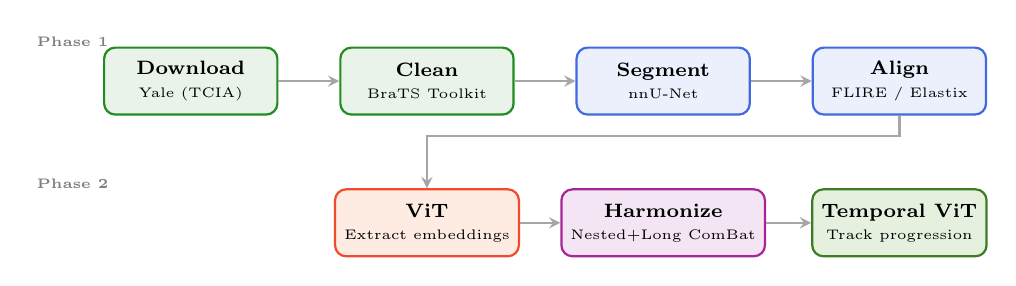
\begin{tikzpicture}[
            box/.style={rectangle, draw=#1, fill=#1!10, thick, minimum height=0.85cm, minimum width=2.2cm, align=center, rounded corners, font=\scriptsize},
            arr/.style={->, thick, >=stealth, color=gray!70},
            lbl/.style={font=\tiny\bfseries, color=gray}
        ]

        % Phase 1 row
        \node[lbl] at (-1.5,0.5) {Phase 1};
        \node[box=ForestGreen] (dl) at (0,0) {\textbf{Download}\\{\tiny Yale (TCIA)}};
        \node[box=ForestGreen] (clean) at (3,0) {\textbf{Clean}\\{\tiny BraTS Toolkit}};
        \node[box=RoyalBlue] (seg) at (6,0) {\textbf{Segment}\\{\tiny nnU-Net}};
        \node[box=RoyalBlue] (reg) at (9,0) {\textbf{Align}\\{\tiny FLIRE / Elastix}};

        \draw[arr] (dl) -- (clean);
        \draw[arr] (clean) -- (seg);
        \draw[arr] (seg) -- (reg);

        % Phase 2 row
        \node[lbl] at (-1.5,-1.3) {Phase 2};
        \node[box=RedOrange] (vit) at (3,-1.8) {\textbf{ViT}\\{\tiny Extract embeddings}};
        \node[box=Mulberry] (harm) at (6,-1.8) {\textbf{Harmonize}\\{\tiny Nested+Long ComBat}};
        \node[box=OliveGreen] (out) at (9,-1.8) {\textbf{Temporal ViT}\\{\tiny Track progression}};

        \draw[arr] (reg) -- ++(0,-0.7) -| (vit);
        \draw[arr] (vit) -- (harm);
        \draw[arr] (harm) -- (out);

        \end{tikzpicture}
    \end{center}

    \vspace{0.2em}

    \begin{columns}
        \begin{column}{0.48\textwidth}
            \begin{block}{\small Phase~1: Data Preparation (10 papers)}
                \scriptsize
                \begin{tabular}{ll}
                    \textbf{Step} & \textbf{Paper} \\
                    \midrule
                    Dataset & Yale (2025), Cyprus (2025) \\
                    Clean & BraTS Toolkit (2020) \\
                    Segment & nnU-Net (2021) \\
                    Align & Registration (2024), FLIRE (2024) \\
                    Harmonize & ComBat Guide, Nested, Long., Valid. \\
                \end{tabular}
            \end{block}
        \end{column}

        \begin{column}{0.48\textwidth}
            \begin{block}{\small Key Design Decision}
                \scriptsize
                \begin{itemize}
                    \item \textbf{ViT extracts features} (not hand-crafted radiomics)
                    \item nnU-Net masks tell ViT \textbf{where} to focus
                    \item ComBat harmonizes \textbf{ViT embeddings}
                    \item $\Rightarrow$ One pipeline, no redundant steps
                \end{itemize}
            \end{block}
        \end{column}
    \end{columns}
\end{frame}

% ============================================================================
% TRANSITION: PART IV
% ============================================================================
\begin{frame}[plain]
    \centering
    \vfill
    \begin{beamercolorbox}[center,shadow=true,rounded=true]{title}
        \usebeamerfont{title}
        \textbf{Part IV: Next Steps}\\
        \vspace{0.5em}
        \large Upcoming Phases
    \end{beamercolorbox}
    \vfill
\end{frame}

% ============================================================================
% SLIDE 20: Upcoming Phases (placeholder)
% ============================================================================
\begin{frame}{Upcoming Research Phases (Papers To Be Reviewed)}
    \begin{columns}
        \begin{column}{0.48\textwidth}
            \begin{block}{\textbf{Phase 2--3:} ViT + Baselines}
                \small
                \begin{itemize}
                    \item CNN baseline models
                    \item Vision Transformers (ViT, Swin)
                    \item Temporal tumor embeddings
                    \item Swin UNETR, UNETR (MONAI)
                \end{itemize}
                \vspace{0.2em}
                {\scriptsize \textit{Papers: to be reviewed next}}
            \end{block}

            \vspace{0.3em}

            \begin{block}{\textbf{Phase 4:} LLM Integration}
                \small
                \begin{itemize}
                    \item Multimodal vision-language models
                    \item Clinical narrative generation
                    \item Candidates: RadFM, LLaVA-Med
                \end{itemize}
                \vspace{0.2em}
                {\scriptsize \textit{Papers: to be reviewed}}
            \end{block}
        \end{column}

        \begin{column}{0.48\textwidth}
            \begin{block}{\textbf{Phase 5:} Video Generation}
                \small
                \begin{itemize}
                    \item Diffusion-based video models
                    \item Counterfactual progression
                    \item Temporal coherence
                    \item Candidates: Video LDM, MVG
                \end{itemize}
                \vspace{0.2em}
                {\scriptsize \textit{Papers: to be reviewed}}
            \end{block}

            \vspace{0.3em}

            \begin{block}{\textbf{Phase 6:} Evaluation}
                \small
                \begin{itemize}
                    \item Quantitative metrics
                    \item Clinical plausibility
                    \item Publication draft
                \end{itemize}
                \vspace{0.2em}
                {\scriptsize \textit{Papers: to be reviewed}}
            \end{block}
        \end{column}
    \end{columns}
\end{frame}

% ============================================================================
% SLIDE 20: Summary & Questions
% ============================================================================
\begin{frame}{Summary}
    \begin{block}{What We Covered}
        \small
        \begin{itemize}
            \item \textbf{Problem:} Current AI is static, unexplainable, and cannot model disease progression
            \item \textbf{Dataset:} Yale (11,884 scans, 1,430 patients) -- chosen for its longitudinal nature
            \item \textbf{Pipeline:} Clean $\to$ Segment $\to$ Align $\to$ ViT Features $\to$ Harmonize
            \item \textbf{Innovation:} ViT extracts features + Nested+Longitudinal ComBat on embeddings
            \item \textbf{Phase~1 literature: 10 papers analyzed}, covering every preprocessing step
        \end{itemize}
    \end{block}

    \begin{alertblock}{Research Gap (Unchanged)}
        \small
        No existing system simultaneously provides explainable reasoning \textbf{and} future progression videos from longitudinal cancer imaging. Our project fills this gap by integrating ViT + LLM + Diffusion.
    \end{alertblock}

    \vspace{0.5em}

    \centering
    \Large \textbf{Thank You! Questions?}
\end{frame}

% ============================================================================
% SLIDE 21: References
% ============================================================================
\begin{frame}[allowframebreaks]{Key References}
    \scriptsize
    \begin{thebibliography}{99}
        \bibitem{yale} Ramachandran et al., ``\href{https://doi.org/10.1038/s41597-025-04360-7}{A longitudinal MRI dataset of brain metastases},'' \textit{Scientific Data}, 2025
        \bibitem{cyprus} Pszczolkowski et al., ``\href{https://doi.org/10.1038/s41597-025-04608-2}{A longitudinal MRI dataset of brain metastases from Cyprus},'' \textit{Scientific Data}, 2025
        \bibitem{brats} Kofler et al., ``\href{https://doi.org/10.3389/fnins.2020.00125}{BraTS Toolkit},'' \textit{Frontiers in Neuroscience}, 2020
        \bibitem{nnunet} Isensee et al., ``\href{https://doi.org/10.1038/s41592-020-01008-z}{nnU-Net},'' \textit{Nature Methods}, 2021
        \bibitem{reg} Estienne et al., ``\href{https://doi.org/10.1016/j.media.2024.103148}{Treatment-aware registration},'' \textit{Medical Image Analysis}, 2024
        \bibitem{flire} Fei et al., ``\href{https://doi.org/10.1002/jmri.29474}{FLIRE},'' \textit{J. Magnetic Resonance Imaging}, 2024
        \bibitem{combat} Orlhac et al., ``\href{https://doi.org/10.2967/jnumed.121.262464}{A Guide to ComBat Harmonization},'' \textit{J. Nuclear Medicine}, 2022
        \bibitem{longcombat} Beer et al., ``\href{https://doi.org/10.1016/j.neuroimage.2020.117129}{Longitudinal ComBat},'' \textit{NeuroImage}, 2020
        \bibitem{valcombat} Richter et al., ``\href{https://doi.org/10.1016/j.ynirp.2022.100136}{Validation of ComBat},'' \textit{NeuroImage: Reports}, 2022
        \bibitem{gencombat} Horng et al., ``\href{https://doi.org/10.1038/s41598-022-08412-9}{Generalized ComBat},'' \textit{Scientific Reports}, 2022
    \end{thebibliography}
\end{frame}

\end{document}
